\begin{frame}{Validação no LTspice: circuitos}
  \begin{columns}[T,onlytextwidth]
    \begin{column}{0.48\textwidth}
      \centering
      \textbf{Circuito 1}

      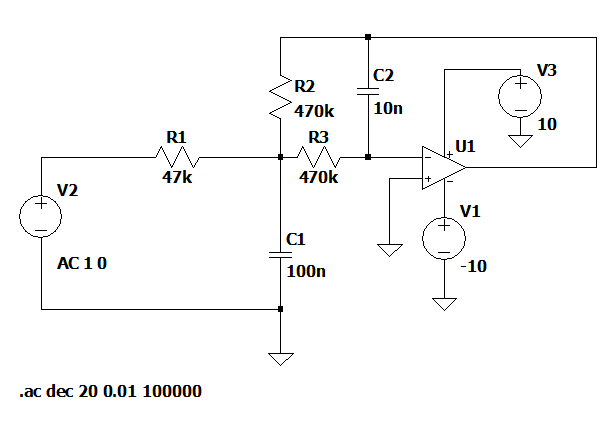
\includegraphics[width=\linewidth,height=0.47\textheight,keepaspectratio]{slides/img/ltspice_circuito_1.png}

      \small $R_1=47\,\mathrm{k}\Omega$, $R_3=470\,\mathrm{k}\Omega$.
    \end{column}
    \begin{column}{0.48\textwidth}
      \centering
      \textbf{Circuito 2}

      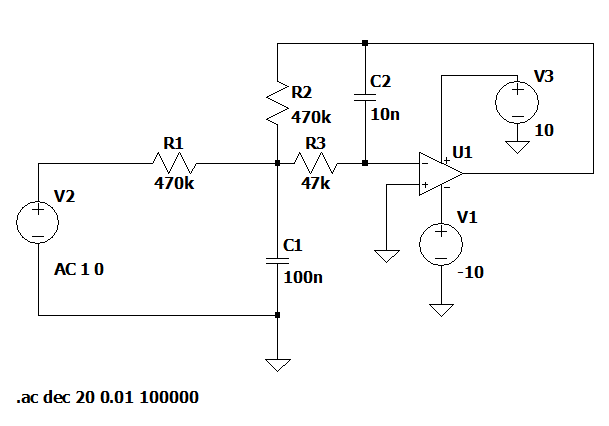
\includegraphics[width=\linewidth,height=0.47\textheight,keepaspectratio]{slides/img/ltspice_circuito_2.png}

      \small $R_1=470\,\mathrm{k}\Omega$, $R_3=47\,\mathrm{k}\Omega$.
    \end{column}
  \end{columns}

  \small
  \begin{block}{Configuração das simulações descritas no relatório}
    Análise AC: amplitude unitária, fase nula e varredura de $0{,}01$ a $10^5\,\mathrm{Hz}$.
    Alimentação do ampop: $\pm10\,\mathrm{V}$.
    Ensaios transitórios: onda quadrada de $0{,}8\,\mathrm{V}$ a $1\,\mathrm{Hz}$
    e de $5\,\mathrm{V}$ a $5\,\mathrm{Hz}$, respectivamente.
  \end{block}
\end{frame}

\begin{frame}{Validação no LTspice: resposta em frequência}
  \small
  \begin{columns}[T,onlytextwidth]
    \begin{column}{0.48\textwidth}
      \centering
      \textbf{Circuito 1}

      \vspace{0.06cm}
      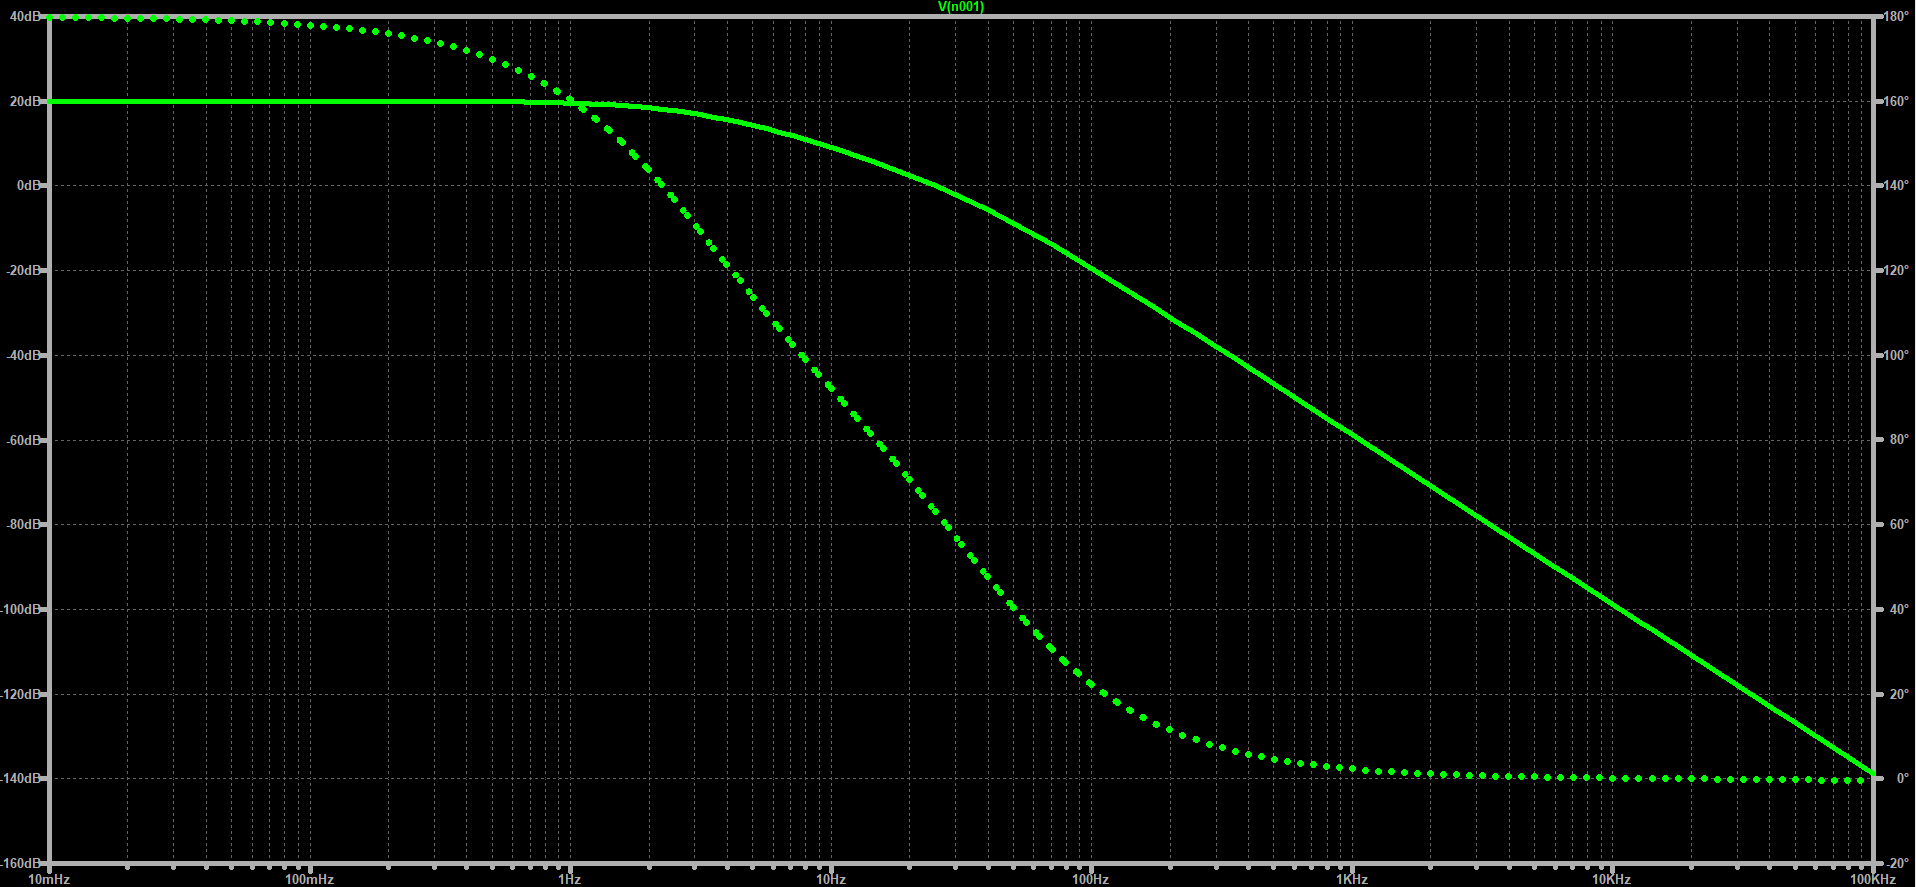
\includegraphics[width=\linewidth]{slides/img/ltspice_bode_1.png}

      \vspace{0.06cm}
      \small Ganho elevado em baixas frequências e atenuação progressiva.
    \end{column}
    \begin{column}{0.48\textwidth}
      \centering
      \textbf{Circuito 2}

      \vspace{0.06cm}
      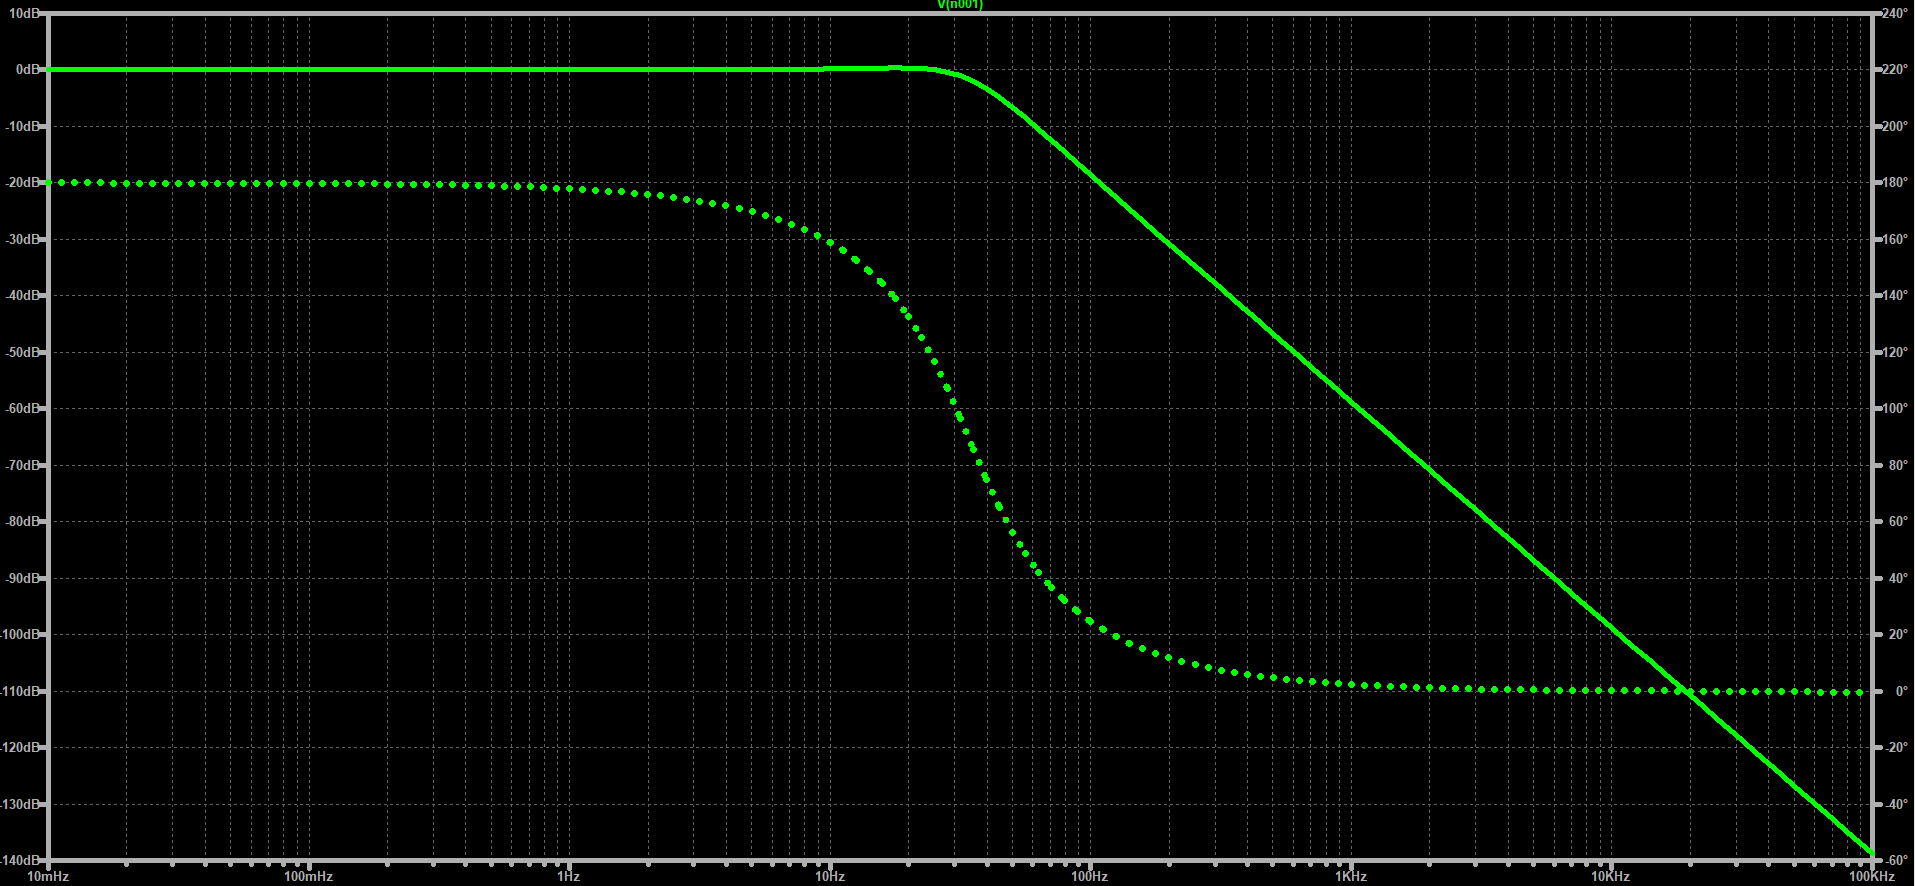
\includegraphics[width=\linewidth]{slides/img/ltspice_bode_2.png}

      \vspace{0.06cm}
      \small Ganho próximo da unidade, pequeno pico e transição mais acentuada.
    \end{column}
  \end{columns}

  \vspace{0.04cm}
  \begin{alertblock}{Comparação com o modelo}
    As curvas reproduzem a característica passa-baixa e o efeito da troca de
    resistores. A comparação é qualitativa: o relatório não apresenta erros
    numéricos da simulação.
  \end{alertblock}
  \centering\scriptsize Capturas originais da prática; magnitude e fase no mesmo painel.
\end{frame}
